\documentclass{article}
\usepackage[utf8]{inputenc}

\usepackage{listings}
\usepackage{algorithm}
\usepackage{algorithmic}
\usepackage{color}
\usepackage{graphicx} %package to manage images

%New colors defined below
\definecolor{codegreen}{rgb}{0,0.6,0}
\definecolor{codegray}{rgb}{0.5,0.5,0.5}
\definecolor{codepurple}{rgb}{0.58,0,0.82}
\definecolor{backcolour}{rgb}{0.95,0.95,0.92}

%Code listing style named "mystyle"
\lstdefinestyle{mystyle}{
  backgroundcolor=\color{backcolour},   commentstyle=\color{codegreen},
  keywordstyle=\color{magenta},
  numberstyle=\tiny\color{codegray},
  stringstyle=\color{codepurple},
  basicstyle=\footnotesize,
  breakatwhitespace=false,         
  breaklines=false,                 
  captionpos=b,                    
  keepspaces=true,                 
  numbers=left,                    
  numbersep=5pt,                  
  showspaces=false,                
  showstringspaces=false,
  showtabs=false,                  
  tabsize=2
}

%"mystyle" code listing set
\lstset{style=mystyle}

\begin{document}
\centerline{\sc \large EECE 7360 Project 3}
\vspace{.5pc}
\centerline{\sc Garrett Goode and Daniel Hullihen}
\centerline{\it Spring 2017}

\section{Introduction}
The subset sum problem (also referred to as the ``exact knapsack problem'')
is defined below.

\textit{Let A = $\{a_1, ..., a_n\}$ represent some set of integers. Given a sum s, find a subset $A' \subset A$ such that
  $$s = \sum_{i=1}^n a_i, for 1 \le i \le n.$$}
In other words, if we are given a list of numbers and some target sum, we want
to find the numbers in the list that would add up to the target sum. Put as a decision
problem, the question would be ``Is there a subset A' of A where the sum of the
elements of A' is s?''

In this project, we developed an implementation of a greedy algorithm
for the subset sum problem, and ran it against a suite of instances to evaluate
the performance of this algorithm.

\section{Greedy Algorithm Implementation}
The implementation of the greedy algorithm that was used for this project is relatively simple.
Below is the psuedocode for the algorithm.

\begin{algorithm}
  \caption{Greedy Algorithm to Solve Subset Sum}
  \label{greedy}
  \begin{algorithmic}
    \STATE{$runningSum \gets 0$}
    \STATE{$subset \gets []$} \COMMENT{Initialize subset to an empty list}
    \FOR{integer i in set S}
    \IF{$runningSum + i \le targetSum$}
    \STATE{$runningSum \gets runningSum + i$}
    \STATE{append i to subset}
    \ENDIF
    \ENDFOR
    \IF{$runningSum == targetSum$}
    \STATE{return subset}
    \ELSE
    \STATE{return NULL}
    \ENDIF
  \end{algorithmic}
\end{algorithm}

We walk through each element of the provided instance, adding numbers so long
as the running sum has not exceeded the target sum. At the end, we check to see
if the running sum matches the target sum; if it does, we have successfully solved
the instance and return the subset of integers. Otherwise we have not solved the instance
and return NULL.

One characteristic of a greedy algorithm is that, once we decide to include an element
to the sum, we never undo the decision. In the case of the subset sum problem, this
can easily cause the algorithm to not find the correct list of elements to use for the sum
since not all combinations of integers in a list are necessarily going to add up to
the target sum. Because of this, a margin of error is introduced where the algorithm
may fall short of the target sum. The upside of this algorithm is the time complexity
improvement: the algorithm visits each element of the set only once, giving the
algorithm a tightly bound time complxity of O(n). This algorithm may be useful for
applications that only need a subset that is within some percent of the target sum,
especially given the improved time complexity over the brute-force solution.

\section{Trivial Case Where the Greedy Algorithm Fails}
Due to the nature of the greedy algorithm explained in the previous section,
we can identify a trivial case where the algorithm will fail. Take for example
the set of integers S below where the target sum is 150.
$$S = \{49, 100, 50\}$$
The greedy algorithm will start from the first element and work its way through
the list, adding numbers so long as the running sum does not go beyond the target sum of 150.
In this case, the algorithm will accept the integers 49 and 100, resulting in a sum of 149.
When it encounters 50, it decides not to add this number since it would bring the running
sum over the target sum. The algorithm has then completed processing the set, but it
has failed to find a solution depite the fact one actually exists.

\section{Results}

The results are presented in Figure~\ref{fig:greedy} below. The vertical axis represents the
input size and the horizontal axis the word length of the elements in bits.

\begin{figure}[h]
\centering
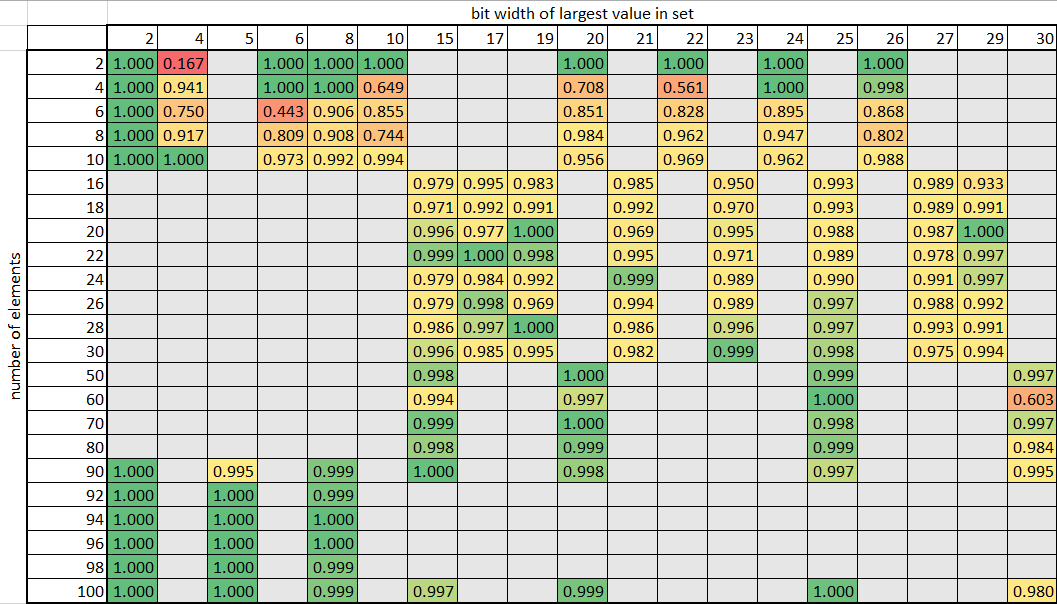
\includegraphics[width=12cm]{P3_margin.png}
\caption{Margin of error for various input size and word length combinations for the greedy algorithm}
\label{fig:greedy}
\end{figure}

Each cell in the above figure is color-coded based on the margin of error
the greedy algorithm had for the given instance. A value of 1 means the algorithm
successfully found a subset whose sum of elements matched the target sum. 
Varying yellow, orange and red elements are cases where the algorithm was more
progressively off from the target sum, with red being the most off/greatest error.

Of the 151 instances that were tested, the greedy algorithm was able to
correctly solve 28 of them, yielding an 18.5\% success rate. Compared to the
exhaustive algorithm, which had a 76\% success rate, the greedy algorithm 
is much less successful despite it's lower time complexity. As a reminder,
Figure~\ref{fig:exhaustive} shows the run-times for the exhaustive algorithm.

\begin{figure}[h]
\centering
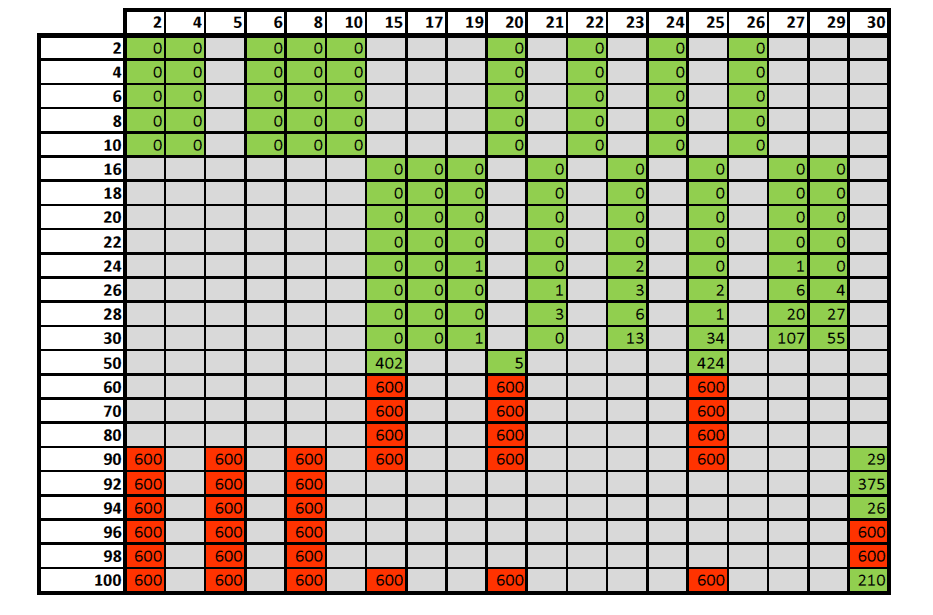
\includegraphics[width=12cm]{P1_res.png}
\caption{Run time for various input size and word length combinations for the exhaustive algorithm}
\label{fig:exhaustive}
\end{figure}

Looking at the results described in Figure~\ref{fig:greedy}, the greedy algorithm was successful
when there were sufficiently few numbers in the set, as well large sets with relatively small numbers.
For example, the majority of the instances with 90+ elements amd a max bit width < 10
passed. This may be due to the fact that, given enough sufficiently small numbers, the algorithm
can work at a small enough granularity and have a better chance to come across a total set
of numbers that can add up to the target. However, as the size of the max value increases,
the margin begins to decrease; the algorithm is less likely to hit the target sum.

The instance where the greedy algorithm had the worst margin was the one with 2 elements and a
max bit width of 4. This is most likely
due to chance. With fewer numbers, there are fewer chances to find other numbers that can add up
to the target sum. It is also a function of the distribution of numbers in the set. If there is a large
distribution of integers and the target sum actually needs the larger value, but the larger value is
at the end of the set, then the algorithm is more likely to not include it and end up with a large
margin of error. One way to possibly correct for this case is by sorting the integers from largest to
smallest before processing them.

There appears to be a sufficiently large area where the margin of error is within a few percent of the target sum,
but the algorithm nevertheless fails. This appears to happen with medium-sized sets (i.e. sets
with more than just a couple elements, but do not have a large number either). This is namely from set sizes
of about 6 to 50. The greedy algorithm is unable to correctly solve the majority of these instances.
This may be due to the fact that there are enough integers where the algorithm can accidentally add one
that will actually never allow the running sum to equal the target sum. Had there been more integers, there
would be more opportunities for the algorithm to find some other integer that could still allow
the algorithm to achieve the target sum.

In general, the amount of margin exhibited by the greedy algorithm seems to come down to how many
subsets actually do exist within the set that
satisfy the target sum, which depends on factors such as the distribution of integers values in the set
and whether a value repeats itself.
For example, for sets with several large and small numbers that are similar to each other, there may
be more subsets that satisfy a given target sum compared to a set with a more even distribution of integers.
Granted, this also depends on the target sum itself. But if there are many subsets that satisfy the
target sum, then the greedy algorithm has a better chance of solving a given instance. 

\end{document}
